\problemname{Confused Lecturer}


Bjarki teaches a course at the university, but is
not particularly organized. He gets especially confused by the fact that the number of lectures
varies from week to week.

The first week, Bjarki holds his $A$ scheduled lectures. But every week except the first, he will assume that the schedule is the same as it was the previous week. So in the second week he holds exactly $A$ lectures again. Because of this,
it sometimes happens that Bjarki lectures to an empty classroom and sometimes that he does not show up when he should. At the end of each week, however, he receives an angry letter from his boss with the times he should have held
lectures, and will instead use those times the following week.

Write a program that, given the number of scheduled lectures over $N$ weeks, outputs the number of
lectures Bjarki holds to empty classrooms and the number of
lectures Bjarki fails to show up for.

\begin{figure}[ht!]
\centering
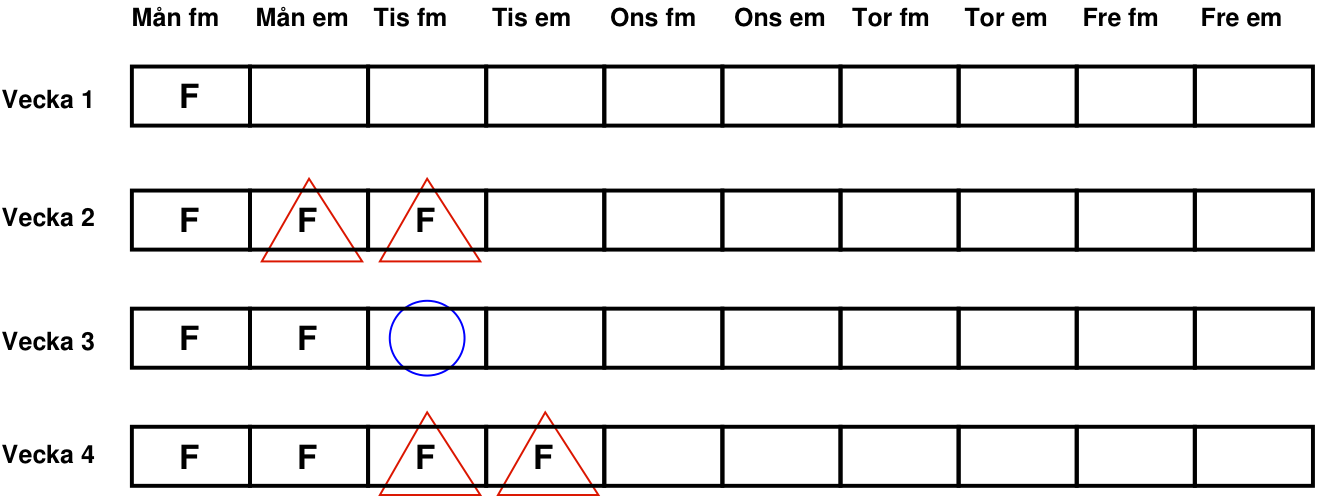
\includegraphics[width=0.8\textwidth]{forelasare.png}
\caption{The schedule in the first example. F marks scheduled lectures. A blue circle marks that Bjarki lectures to an empty classroom and a red triangle marks that he does not show up. {\bf Explanation:} The first week Bjarki always knows which
lectures he should hold. The following week he thinks he should only
hold one lecture, and therefore misses two. The third week he holds
three lectures, one of which is to an empty classroom, and the last week he misses two
lectures. In total he has held 1 empty lecture and missed 4 lectures.} 
\label{overflow}
\end{figure}


\section*{Input}

First comes the number $N$ on its own line, where $1\le N \le 9$. Then follow $N$ integers, the number of
scheduled lectures during each of the weeks.

There can never be more than 10 lectures during a week and the time slots are always filled from the beginning of the week without gaps (see the figure above). 

\section*{Output}
Output the number of empty lectures Bjarki has held, a space,
then the number of lectures Bjarki has missed.
